\chapter{U-Net architecture}
\label{ch:u_net_architecture}

In the few years, deep convolutional networks have outperformed the state of the art in many visual recognition tasks. While convolutional networks have already existed for a long time their success was limited due to the size of the available training sets and the size of the considered networks.

The typical use of convolutional networks is on classification tasks, where the output to an image is a single class label. However, in many visual tasks, especially in biomedical image processing, the desired output should include localization, i.e., a class label is supposed to be assigned to each pixel. Moreover, thousands of training images are usually beyond reach in biomedical tasks. Hence trained a network in a sliding-window setup to predict the class label of each pixel by providing a local region (patch) around that pixel as input. First, this network can localize. Secondly, the training data in terms of patches is much larger than the number of training images.

U-net was originally invented and first used for biomedical image segmentation. Its architecture can be broadly thought of as an encoder network followed by a decoder network. Unlike classification where the end result of the the deep network is the only important thing, semantic segmentation not only requires discrimination at pixel level but also a mechanism to project the discriminative features learnt at different stages of the encoder onto the pixel space. 


The encoder is the first half in the architecture diagram \ref{fig:unet}. It usually is a pre-trained classification network like VGG/ResNet where you apply convolution blocks followed by a maxpool downsampling to encode the input image into feature representations at multiple different levels.

The decoder is the second half of the architecture. The goal is to semantically project the discriminative features (lower resolution) learnt by the encoder onto the pixel space (higher resolution) to get a dense classification. The decoder consists of upsampling and concatenation followed by regular convolution operations.

\begin{figure}[!h]
\begin{center}
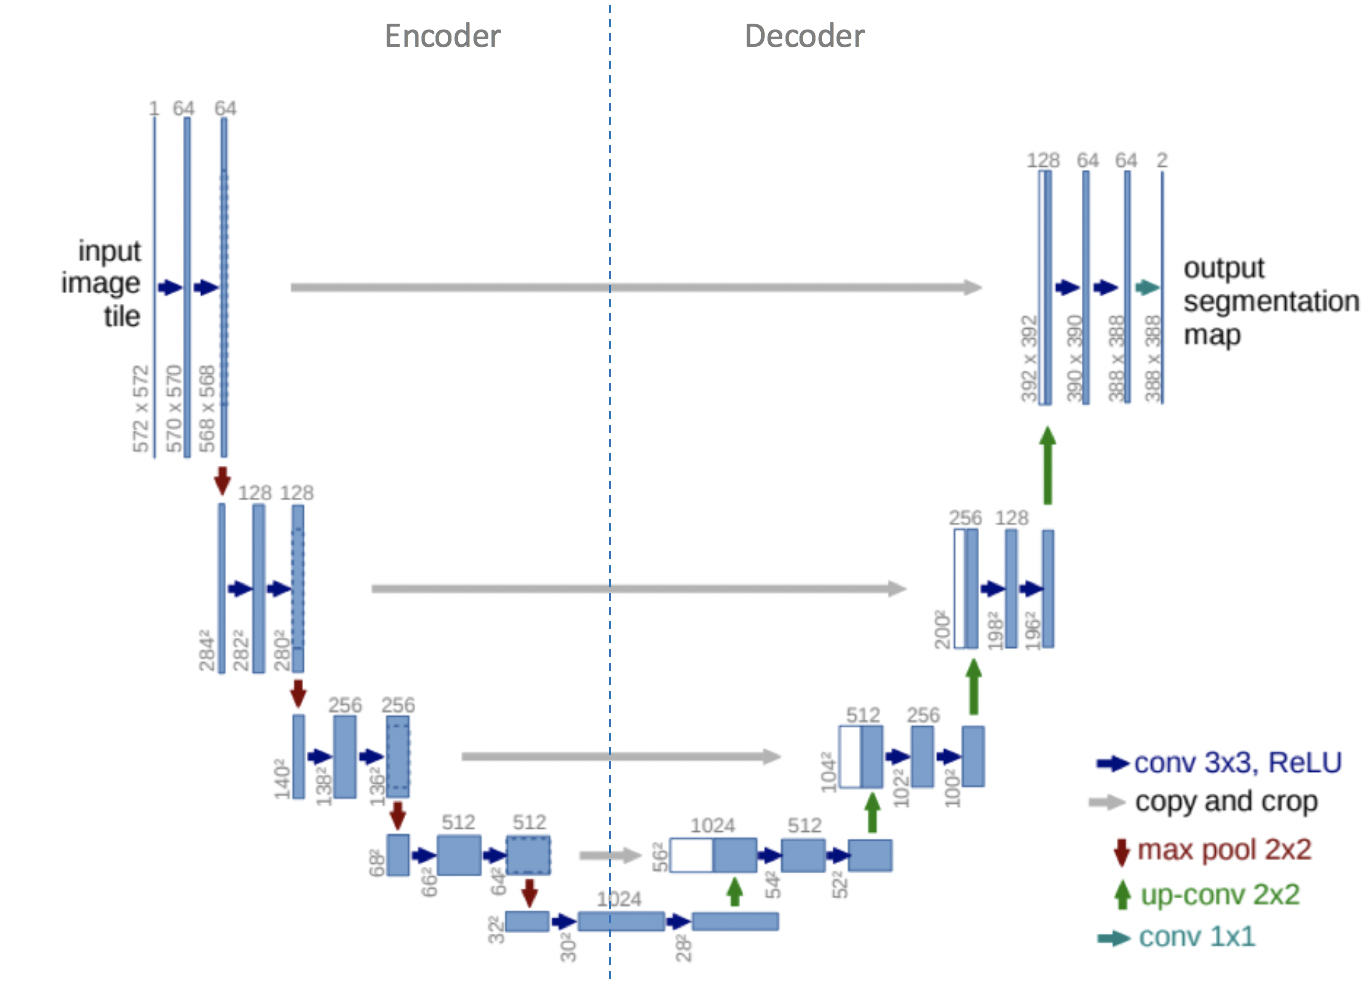
\includegraphics[width=.7\linewidth]{images/unet.png}
\caption {U-net architecture. Blue boxes represent multi-channel feature maps, while while boxes represent copied feature maps. The arrows of different colors represent different operations.} 
\label{fig:unet}
\end{center}
\end{figure}

The intuition is that we would like to restore the condensed feature map to the original size of the input image, therefore we expand the feature dimensions. Upsampling is also referred to as transposed convolution, upconvolution, or deconvolution. There are a few ways of upsampling such as Nearest Neighbor, Bilinear Interpolation, and Transposed Convolution from simplest to more complex.

In summary, unlike classification where the end result of the very deep network is the only important thing, semantic segmentation not only requires discrimination at pixel level but also a mechanism to project the discriminative features learnt at different stages of the encoder onto the pixel space.